\documentclass[11pt]{article}
\usepackage[textwidth=18.0cm, textheight=23.0cm, top=2.0cm]{geometry}
\usepackage{pst-all}
\usepackage{amssymb}
\usepackage{tikz}
\usepackage{underscore}\begin{document}
\pagestyle{empty}


ClassName: \underline{\textbf{Class_07.2bp-19}}
\par
BinSize: \underline{\textbf{100 × 100}}
\par
ReduceSize: \underline{\textbf{100 × 100}}
\par
TypeNum: \underline{\textbf{39}}
\par
Num: \underline{\textbf{40}}
\par
OutS: \underline{\textbf{130000}}
\par
InS: \underline{\textbf{102031}}
\par
Rate: \underline{\textbf{0.785}}
\par
UB: \underline{\textbf{13}}
\par
LB0: \underline{\textbf{13}}
\par
LB: \underline{\textbf{13}}
\par
LBWithCut: \underline{\textbf{13}}
\par
NodeCut: \underline{\textbf{0}}
\par
ExtendedNodeCnt: \underline{\textbf{1}}
\par
GenNodeCnt: \underline{\textbf{1}}
\par
PrimalNode: \underline{\textbf{0}}
\par
ColumnCount: \underline{\textbf{13}}
\par
TotalCutCount: \underline{\textbf{0}}
\par
RootCutCount: \underline{\textbf{0}}
\par
LPSolverCnt: \underline{\textbf{1}}
\par
PricingSolverCnt: \underline{\textbf{0}}
\par
BranchAndBoundNum: \underline{\textbf{1}}
\par
isOpt: \underline{\textbf{true}}
\par
TimeOnInitSolution: \underline{\textbf{600.000 s}}
\par
TimeOnPrimal: \underline{\textbf{0.000 s}}
\par
TimeOnPricing: \underline{\textbf{0.000 s}}
\par
TimeOnRmp: \underline{\textbf{0.062 s}}
\par
TotalTime: \underline{\textbf{600.343 s}}
\par
\newpage


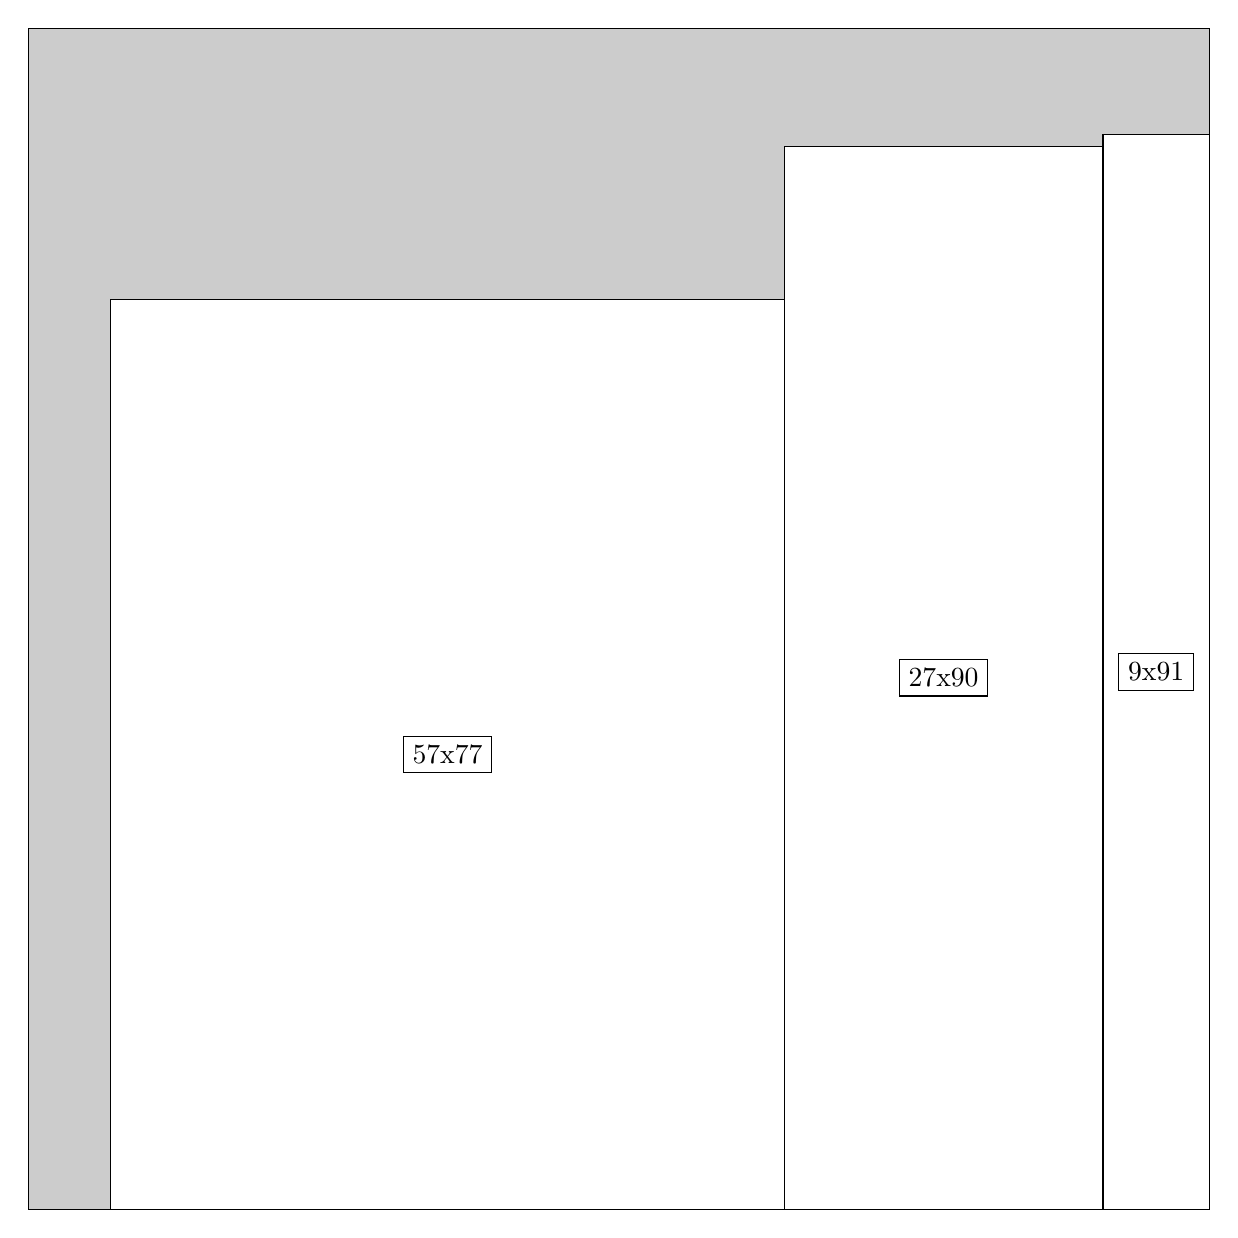
\begin{tikzpicture}[shorten >=1pt,scale=1.0,every node/.style={scale=1.0},->]
\tikzstyle{vertex}=[circle,fill=black!25,minimum size=14pt,inner sep=0pt]
\filldraw[fill=gray!40!white, draw=black] (0,0) rectangle (15.0,15.0);
\foreach \name/\x/\y/\w/\h in {9x91/13.65/0.0/1.3499999999999999/13.65,27x90/9.6/0.0/4.05/13.5,57x77/1.05/0.0/8.549999999999999/11.549999999999999}
\filldraw[fill=white!40!white, draw=black] (\x,\y) rectangle node[draw] (\name) {\name} ++(\w,\h);
\end{tikzpicture}


w =9 , h =91 , x =91 , y =0 , v =819
\par
w =27 , h =90 , x =64 , y =0 , v =2430
\par
w =57 , h =77 , x =7 , y =0 , v =4389
\par
\newpage


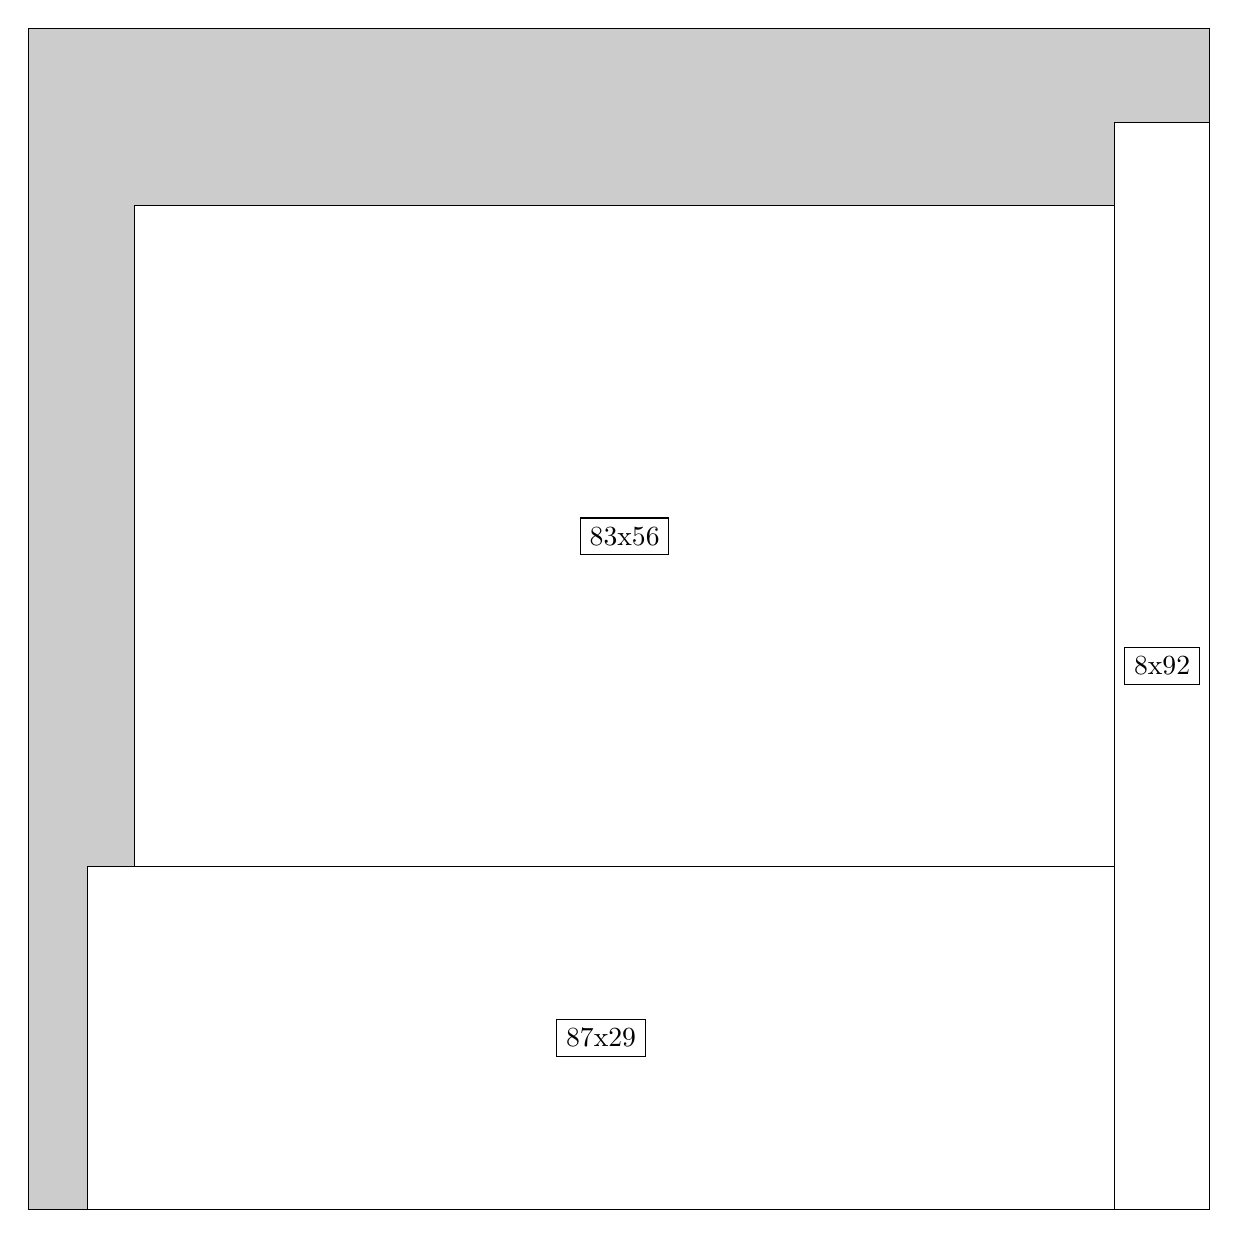
\begin{tikzpicture}[shorten >=1pt,scale=1.0,every node/.style={scale=1.0},->]
\tikzstyle{vertex}=[circle,fill=black!25,minimum size=14pt,inner sep=0pt]
\filldraw[fill=gray!40!white, draw=black] (0,0) rectangle (15.0,15.0);
\foreach \name/\x/\y/\w/\h in {8x92/13.799999999999999/0.0/1.2/13.799999999999999,87x29/0.75/0.0/13.049999999999999/4.35,83x56/1.3499999999999999/4.35/12.45/8.4}
\filldraw[fill=white!40!white, draw=black] (\x,\y) rectangle node[draw] (\name) {\name} ++(\w,\h);
\end{tikzpicture}


w =8 , h =92 , x =92 , y =0 , v =736
\par
w =87 , h =29 , x =5 , y =0 , v =2523
\par
w =83 , h =56 , x =9 , y =29 , v =4648
\par
\newpage


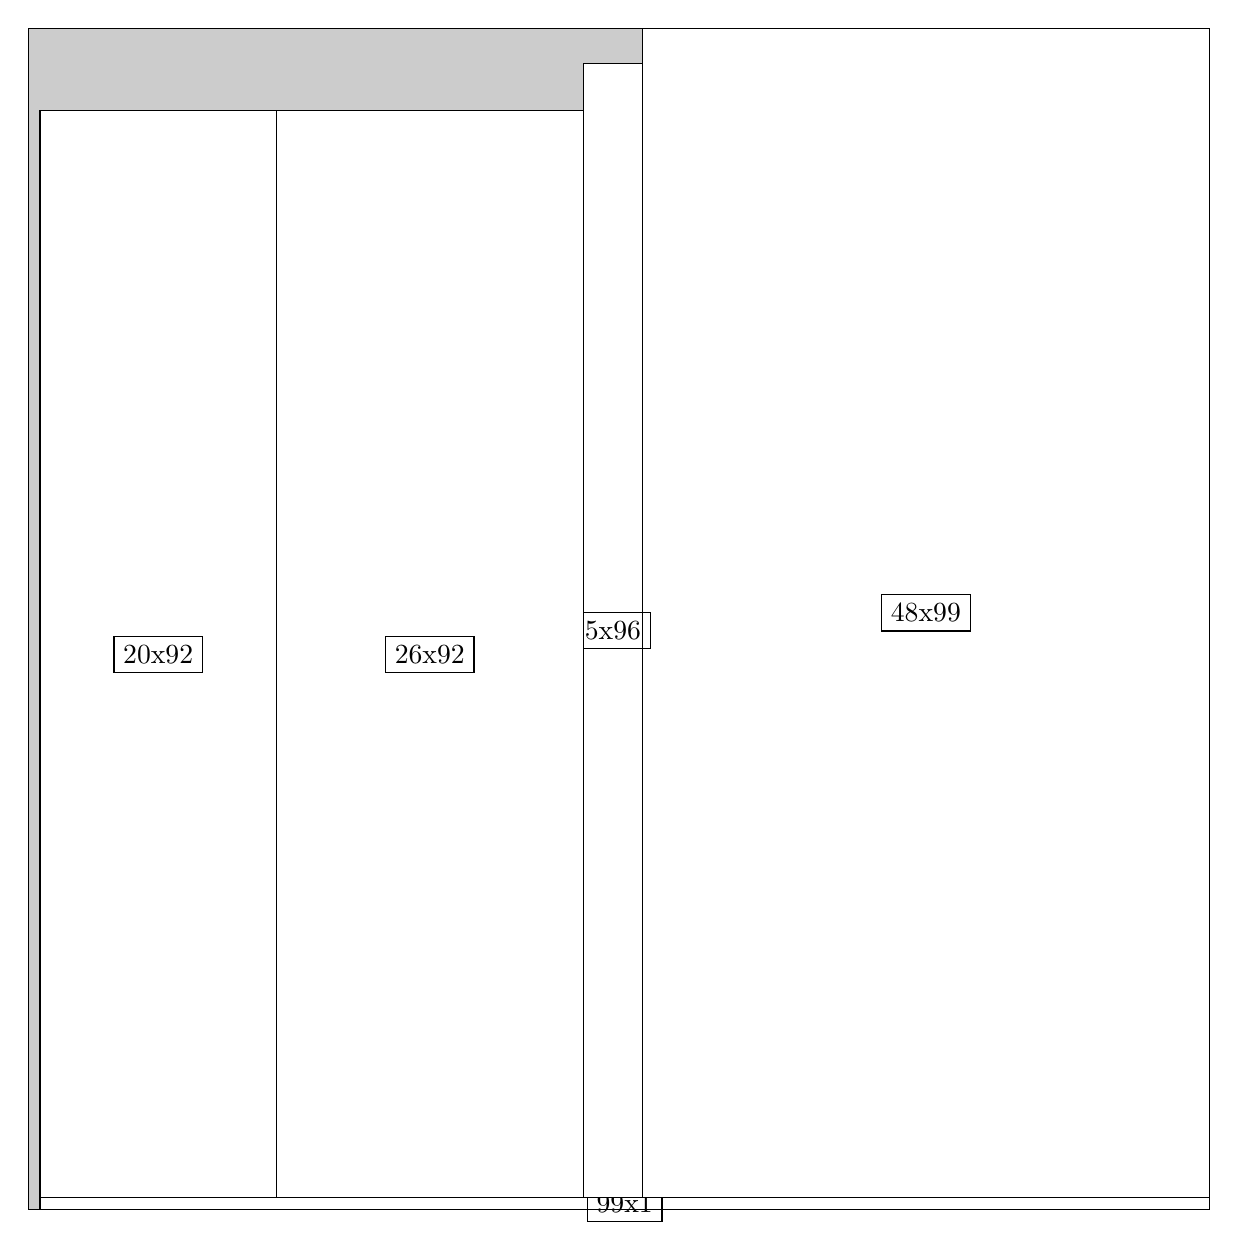
\begin{tikzpicture}[shorten >=1pt,scale=1.0,every node/.style={scale=1.0},->]
\tikzstyle{vertex}=[circle,fill=black!25,minimum size=14pt,inner sep=0pt]
\filldraw[fill=gray!40!white, draw=black] (0,0) rectangle (15.0,15.0);
\foreach \name/\x/\y/\w/\h in {99x1/0.15/0.0/14.85/0.15,48x99/7.8/0.15/7.199999999999999/14.85,5x96/7.05/0.15/0.75/14.399999999999999,26x92/3.15/0.15/3.9/13.799999999999999,20x92/0.15/0.15/3.0/13.799999999999999}
\filldraw[fill=white!40!white, draw=black] (\x,\y) rectangle node[draw] (\name) {\name} ++(\w,\h);
\end{tikzpicture}


w =99 , h =1 , x =1 , y =0 , v =99
\par
w =48 , h =99 , x =52 , y =1 , v =4752
\par
w =5 , h =96 , x =47 , y =1 , v =480
\par
w =26 , h =92 , x =21 , y =1 , v =2392
\par
w =20 , h =92 , x =1 , y =1 , v =1840
\par
\newpage


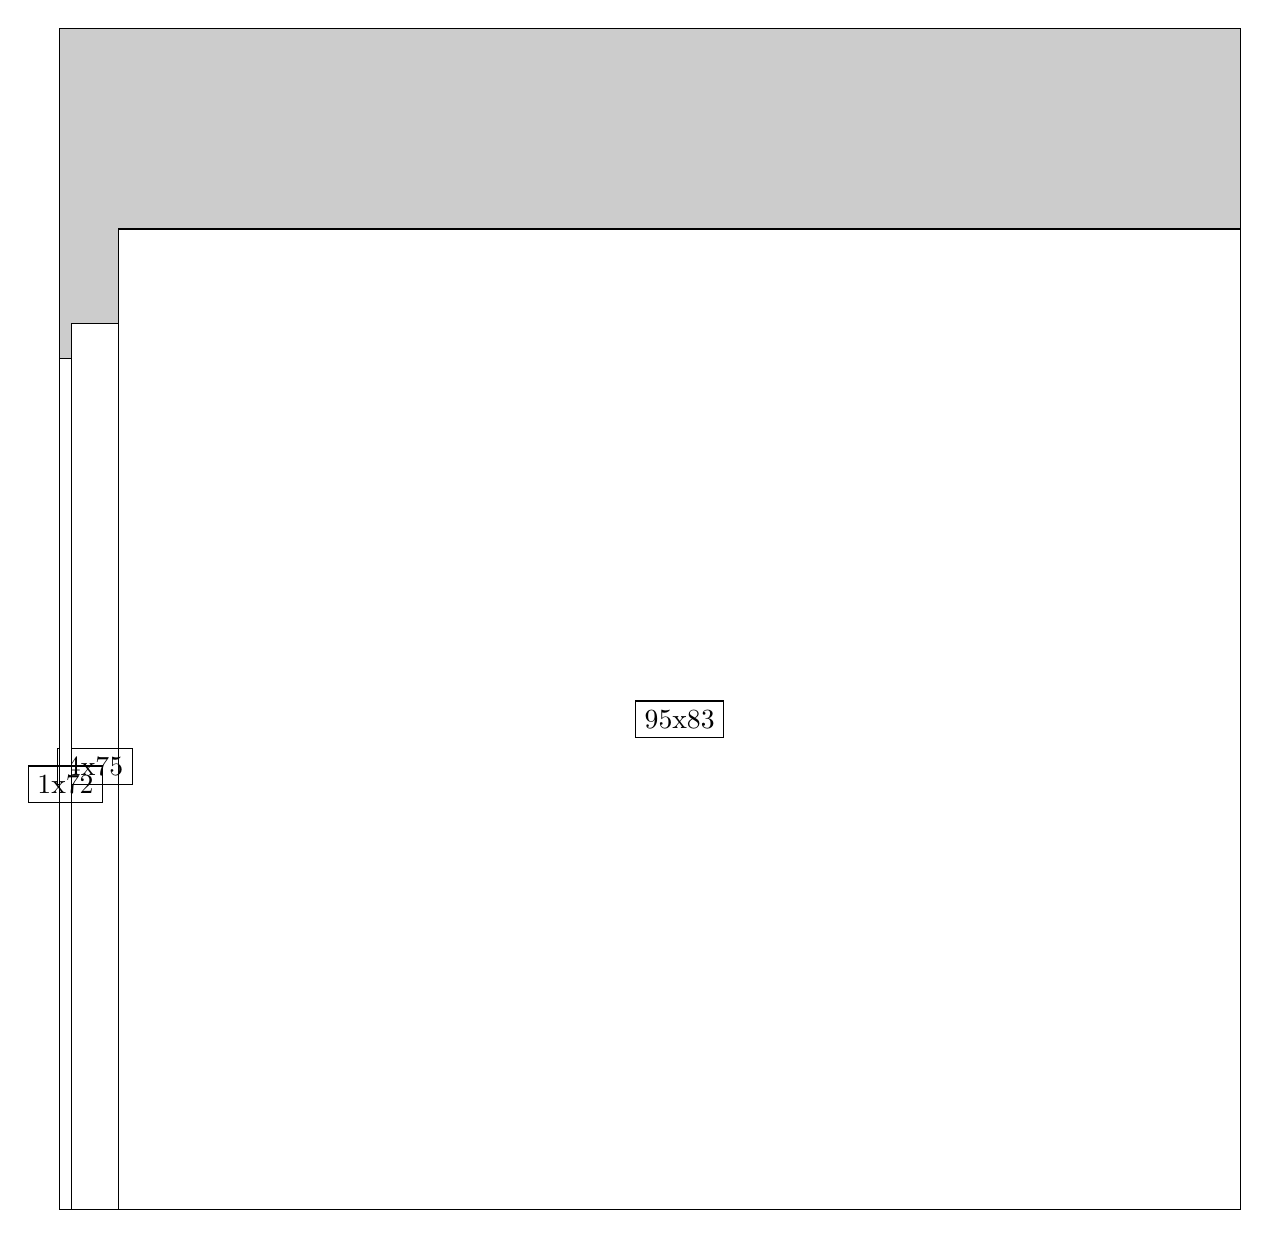
\begin{tikzpicture}[shorten >=1pt,scale=1.0,every node/.style={scale=1.0},->]
\tikzstyle{vertex}=[circle,fill=black!25,minimum size=14pt,inner sep=0pt]
\filldraw[fill=gray!40!white, draw=black] (0,0) rectangle (15.0,15.0);
\foreach \name/\x/\y/\w/\h in {95x83/0.75/0.0/14.25/12.45,4x75/0.15/0.0/0.6/11.25,1x72/0.0/0.0/0.15/10.799999999999999}
\filldraw[fill=white!40!white, draw=black] (\x,\y) rectangle node[draw] (\name) {\name} ++(\w,\h);
\end{tikzpicture}


w =95 , h =83 , x =5 , y =0 , v =7885
\par
w =4 , h =75 , x =1 , y =0 , v =300
\par
w =1 , h =72 , x =0 , y =0 , v =72
\par
\newpage


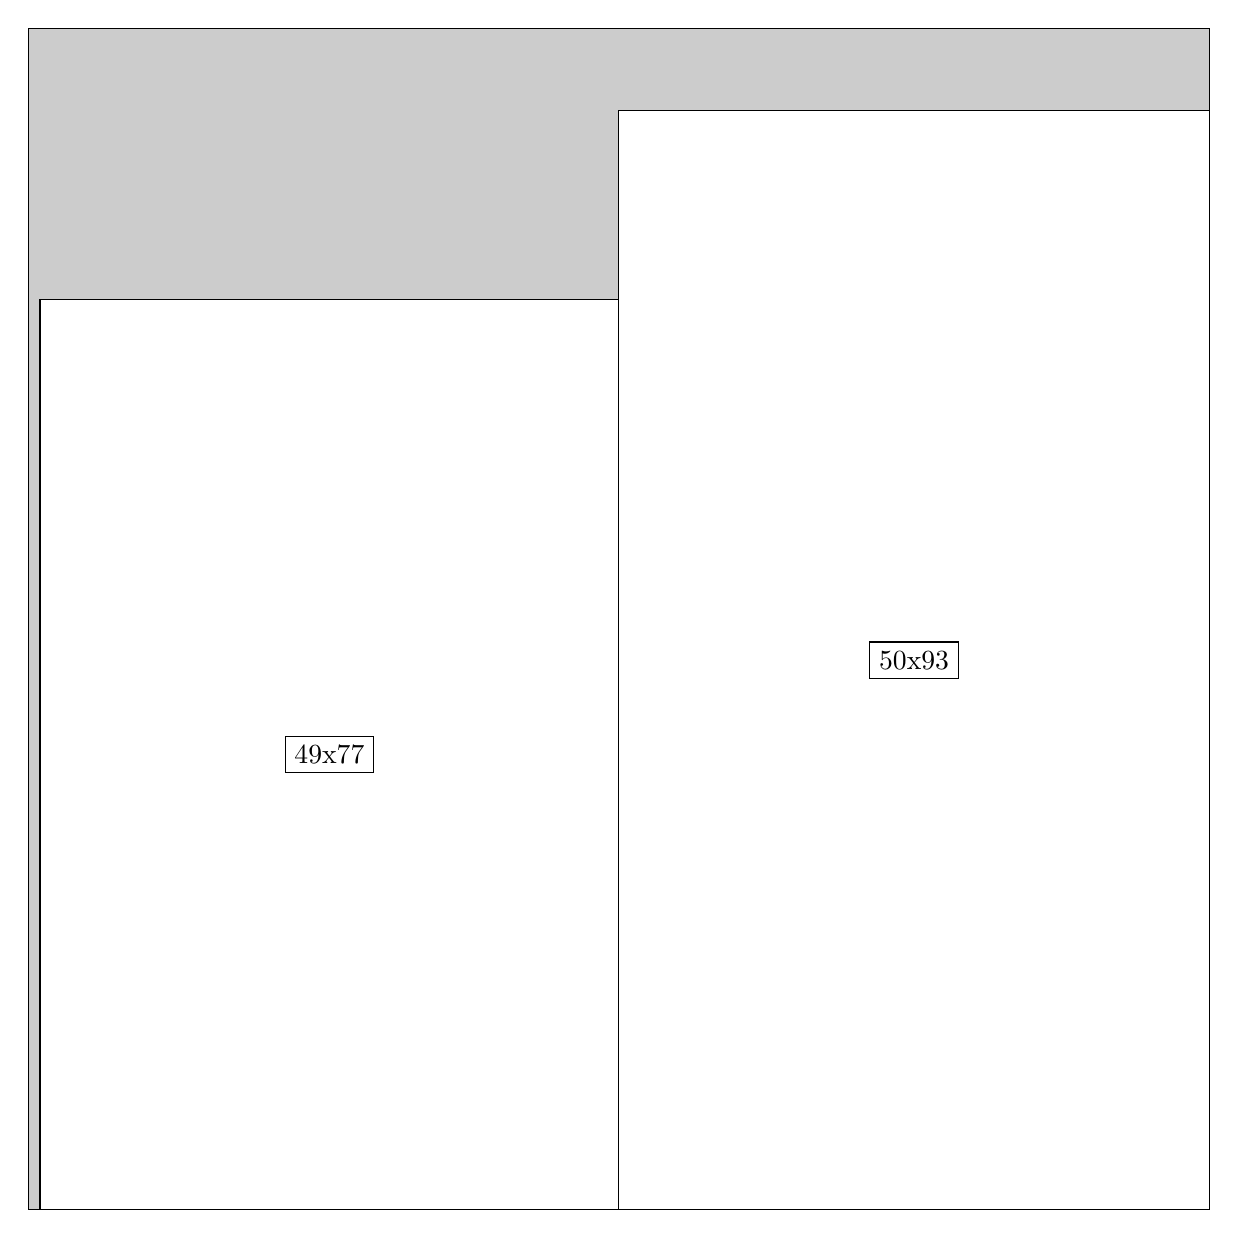
\begin{tikzpicture}[shorten >=1pt,scale=1.0,every node/.style={scale=1.0},->]
\tikzstyle{vertex}=[circle,fill=black!25,minimum size=14pt,inner sep=0pt]
\filldraw[fill=gray!40!white, draw=black] (0,0) rectangle (15.0,15.0);
\foreach \name/\x/\y/\w/\h in {50x93/7.5/0.0/7.5/13.95,49x77/0.15/0.0/7.35/11.549999999999999}
\filldraw[fill=white!40!white, draw=black] (\x,\y) rectangle node[draw] (\name) {\name} ++(\w,\h);
\end{tikzpicture}


w =50 , h =93 , x =50 , y =0 , v =4650
\par
w =49 , h =77 , x =1 , y =0 , v =3773
\par
\newpage


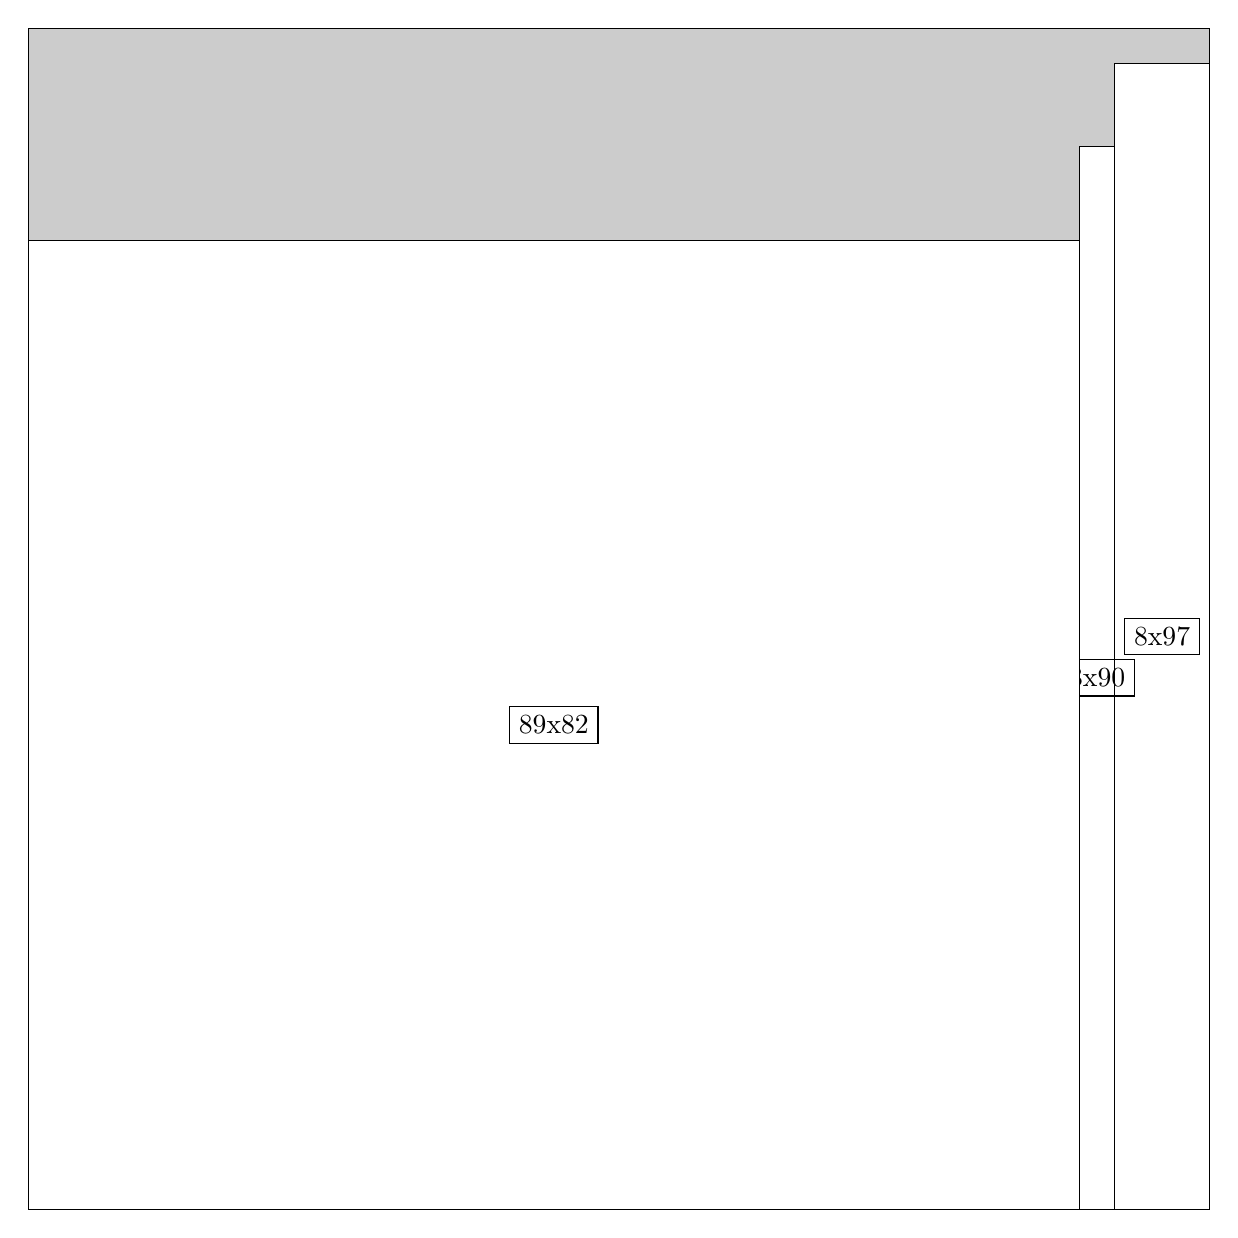
\begin{tikzpicture}[shorten >=1pt,scale=1.0,every node/.style={scale=1.0},->]
\tikzstyle{vertex}=[circle,fill=black!25,minimum size=14pt,inner sep=0pt]
\filldraw[fill=gray!40!white, draw=black] (0,0) rectangle (15.0,15.0);
\foreach \name/\x/\y/\w/\h in {8x97/13.799999999999999/0.0/1.2/14.549999999999999,3x90/13.35/0.0/0.44999999999999996/13.5,89x82/0.0/0.0/13.35/12.299999999999999}
\filldraw[fill=white!40!white, draw=black] (\x,\y) rectangle node[draw] (\name) {\name} ++(\w,\h);
\end{tikzpicture}


w =8 , h =97 , x =92 , y =0 , v =776
\par
w =3 , h =90 , x =89 , y =0 , v =270
\par
w =89 , h =82 , x =0 , y =0 , v =7298
\par
\newpage


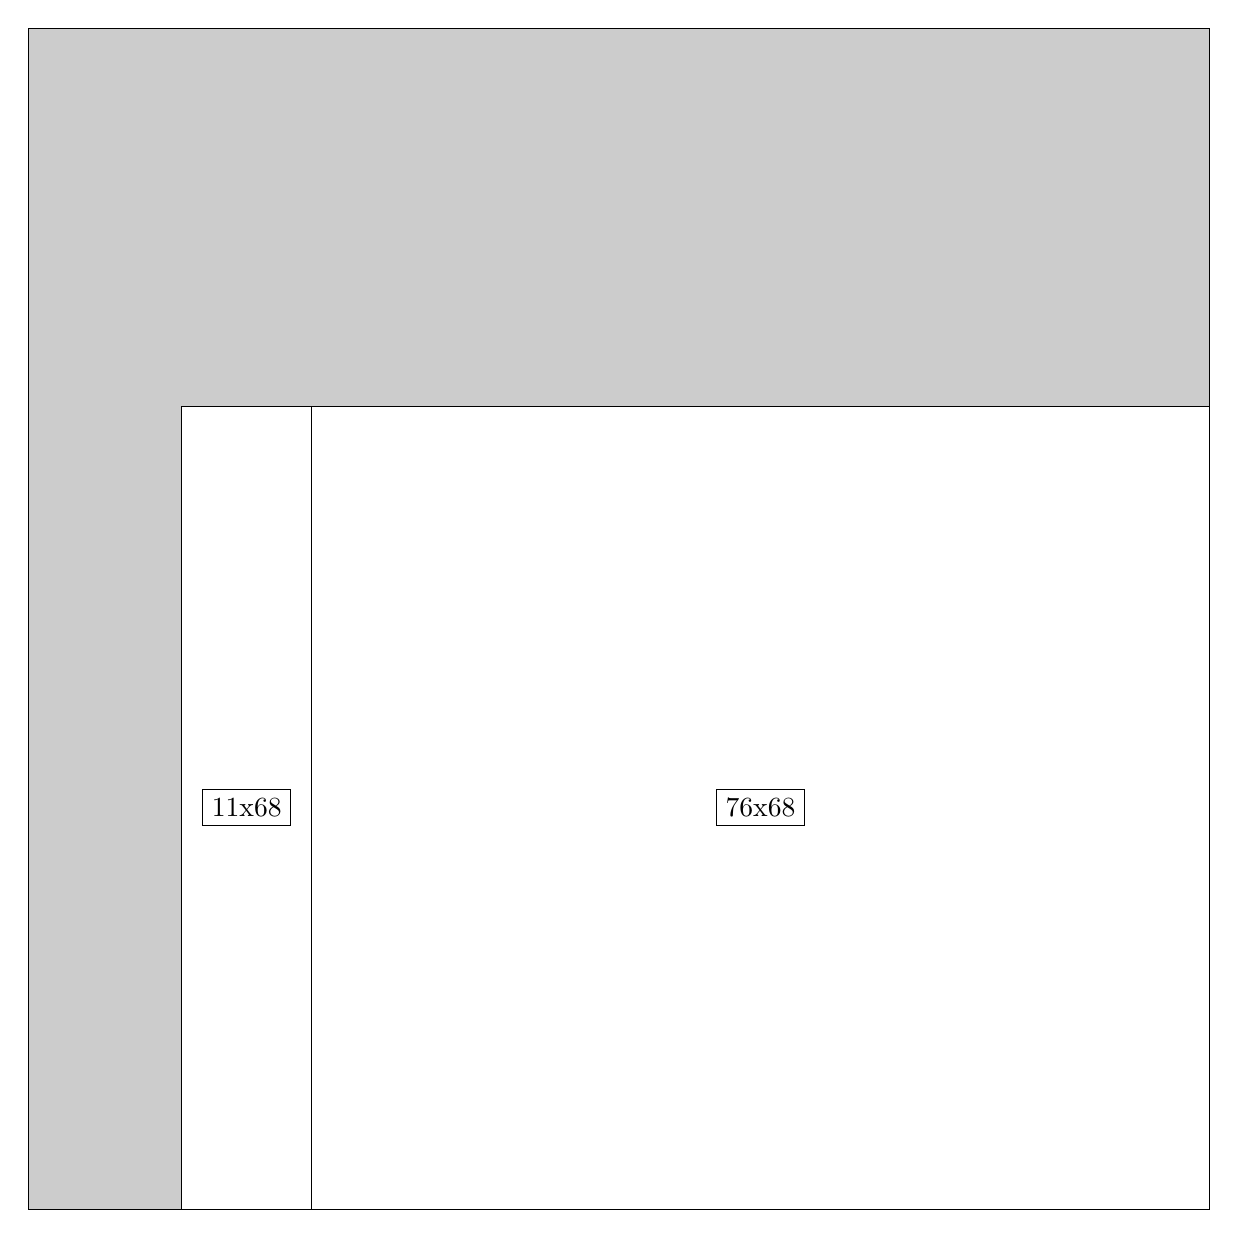
\begin{tikzpicture}[shorten >=1pt,scale=1.0,every node/.style={scale=1.0},->]
\tikzstyle{vertex}=[circle,fill=black!25,minimum size=14pt,inner sep=0pt]
\filldraw[fill=gray!40!white, draw=black] (0,0) rectangle (15.0,15.0);
\foreach \name/\x/\y/\w/\h in {76x68/3.5999999999999996/0.0/11.4/10.2,11x68/1.95/0.0/1.65/10.2}
\filldraw[fill=white!40!white, draw=black] (\x,\y) rectangle node[draw] (\name) {\name} ++(\w,\h);
\end{tikzpicture}


w =76 , h =68 , x =24 , y =0 , v =5168
\par
w =11 , h =68 , x =13 , y =0 , v =748
\par
\newpage


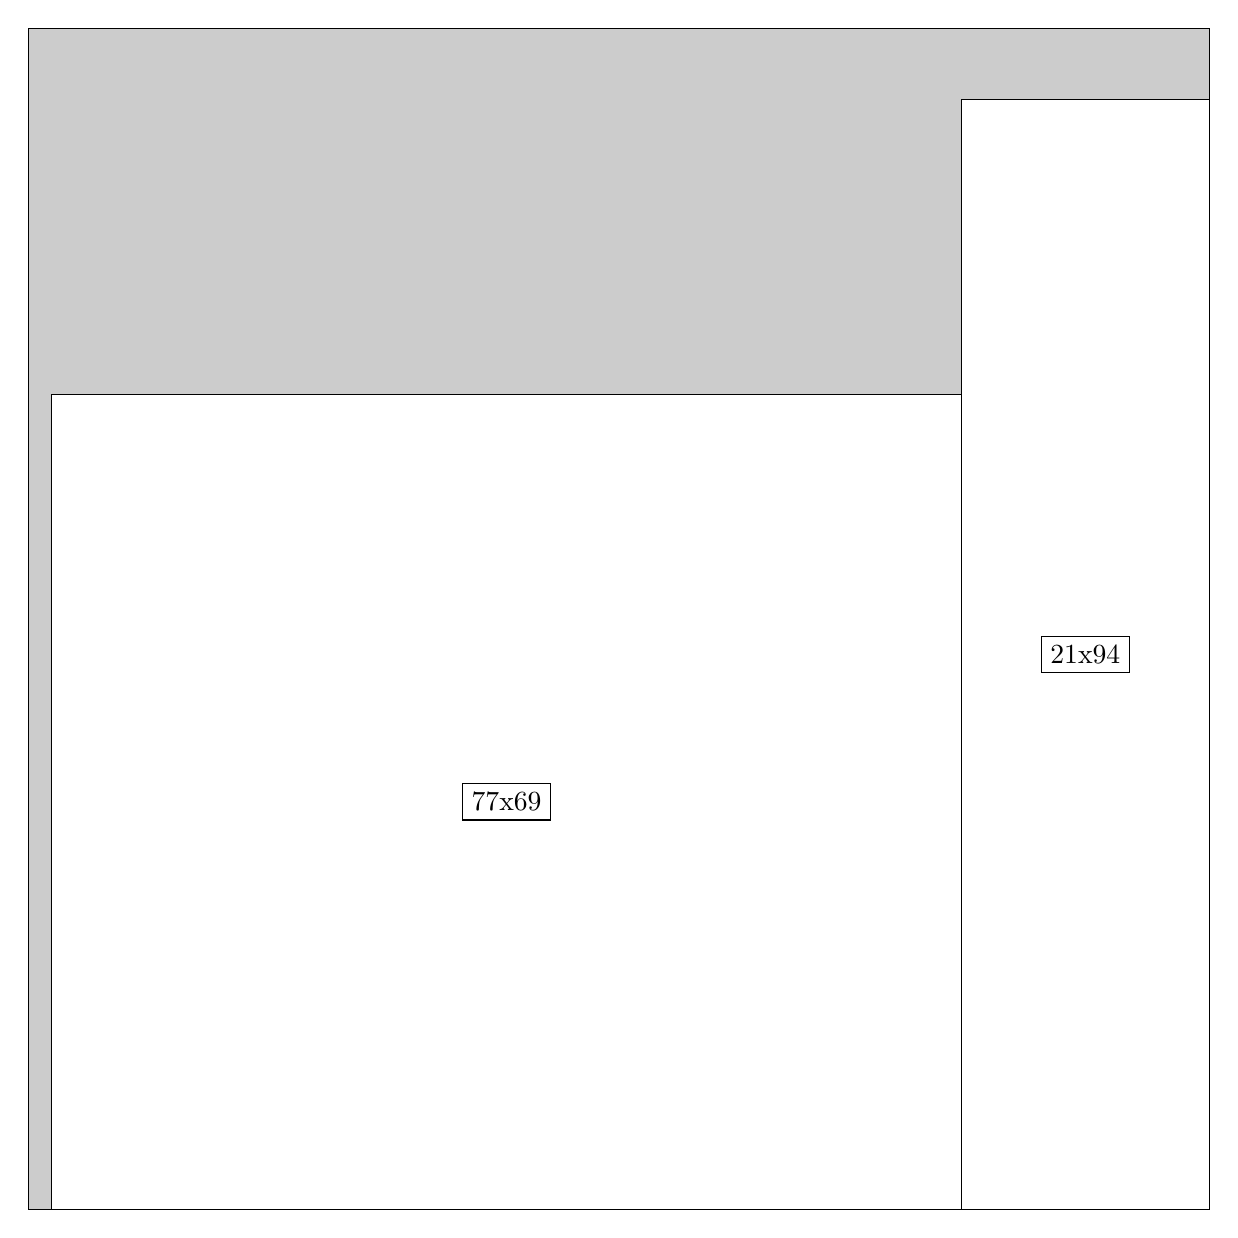
\begin{tikzpicture}[shorten >=1pt,scale=1.0,every node/.style={scale=1.0},->]
\tikzstyle{vertex}=[circle,fill=black!25,minimum size=14pt,inner sep=0pt]
\filldraw[fill=gray!40!white, draw=black] (0,0) rectangle (15.0,15.0);
\foreach \name/\x/\y/\w/\h in {21x94/11.85/0.0/3.15/14.1,77x69/0.3/0.0/11.549999999999999/10.35}
\filldraw[fill=white!40!white, draw=black] (\x,\y) rectangle node[draw] (\name) {\name} ++(\w,\h);
\end{tikzpicture}


w =21 , h =94 , x =79 , y =0 , v =1974
\par
w =77 , h =69 , x =2 , y =0 , v =5313
\par
\newpage


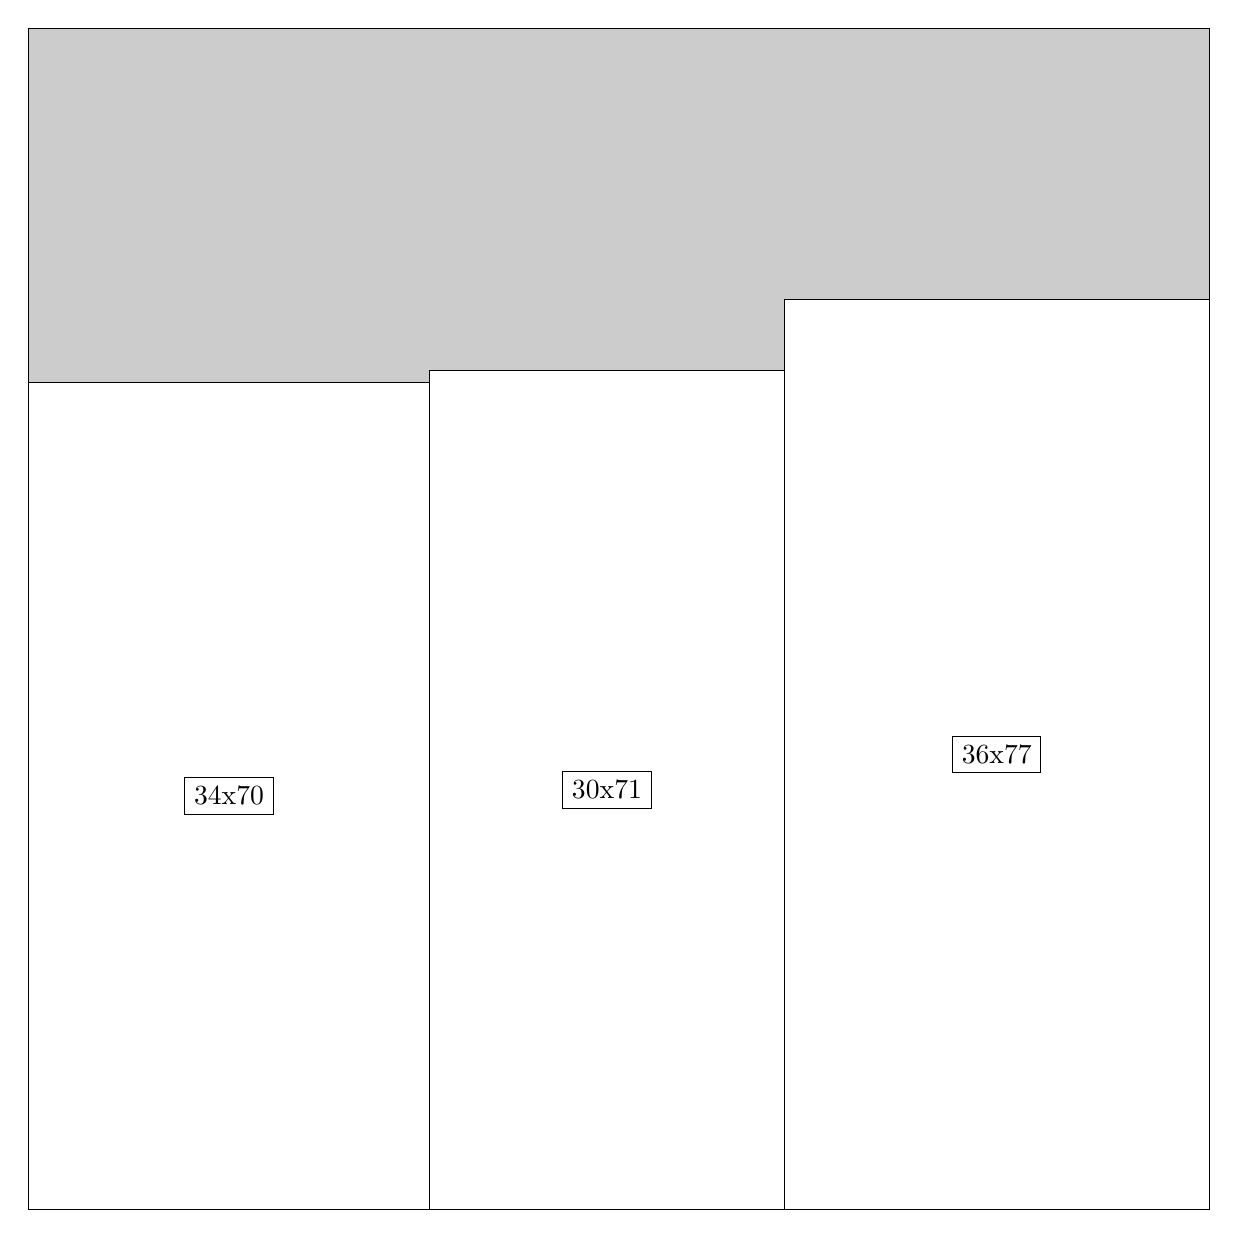
\begin{tikzpicture}[shorten >=1pt,scale=1.0,every node/.style={scale=1.0},->]
\tikzstyle{vertex}=[circle,fill=black!25,minimum size=14pt,inner sep=0pt]
\filldraw[fill=gray!40!white, draw=black] (0,0) rectangle (15.0,15.0);
\foreach \name/\x/\y/\w/\h in {36x77/9.6/0.0/5.3999999999999995/11.549999999999999,30x71/5.1/0.0/4.5/10.65,34x70/0.0/0.0/5.1/10.5}
\filldraw[fill=white!40!white, draw=black] (\x,\y) rectangle node[draw] (\name) {\name} ++(\w,\h);
\end{tikzpicture}


w =36 , h =77 , x =64 , y =0 , v =2772
\par
w =30 , h =71 , x =34 , y =0 , v =2130
\par
w =34 , h =70 , x =0 , y =0 , v =2380
\par
\newpage


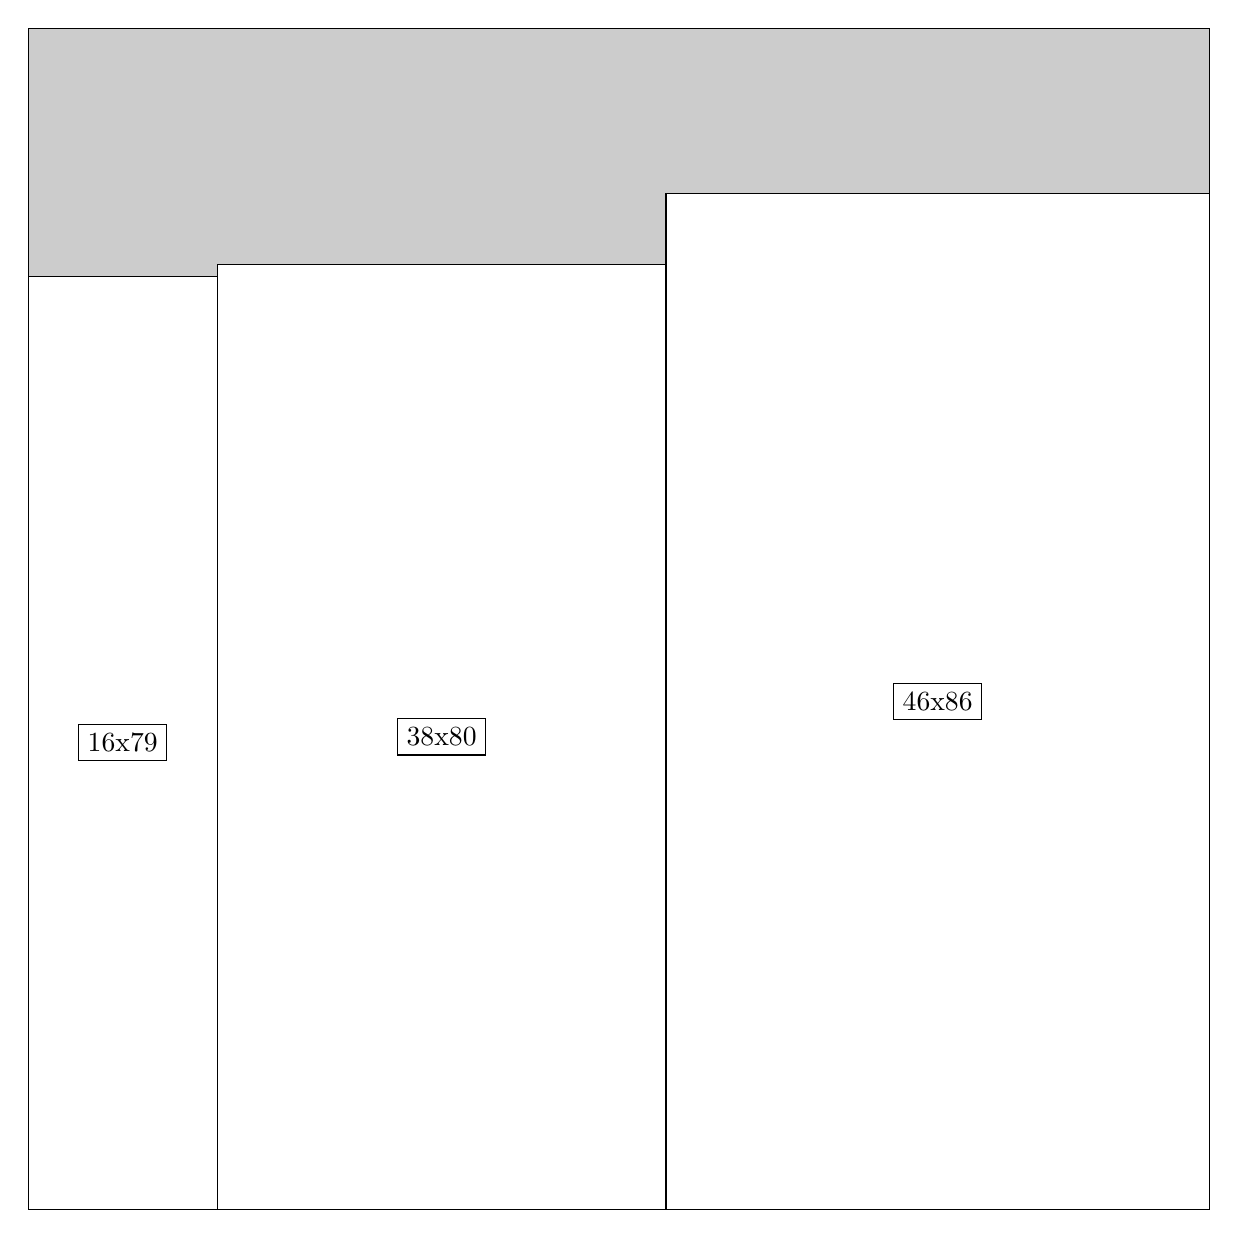
\begin{tikzpicture}[shorten >=1pt,scale=1.0,every node/.style={scale=1.0},->]
\tikzstyle{vertex}=[circle,fill=black!25,minimum size=14pt,inner sep=0pt]
\filldraw[fill=gray!40!white, draw=black] (0,0) rectangle (15.0,15.0);
\foreach \name/\x/\y/\w/\h in {46x86/8.1/0.0/6.8999999999999995/12.9,38x80/2.4/0.0/5.7/12.0,16x79/0.0/0.0/2.4/11.85}
\filldraw[fill=white!40!white, draw=black] (\x,\y) rectangle node[draw] (\name) {\name} ++(\w,\h);
\end{tikzpicture}


w =46 , h =86 , x =54 , y =0 , v =3956
\par
w =38 , h =80 , x =16 , y =0 , v =3040
\par
w =16 , h =79 , x =0 , y =0 , v =1264
\par
\newpage


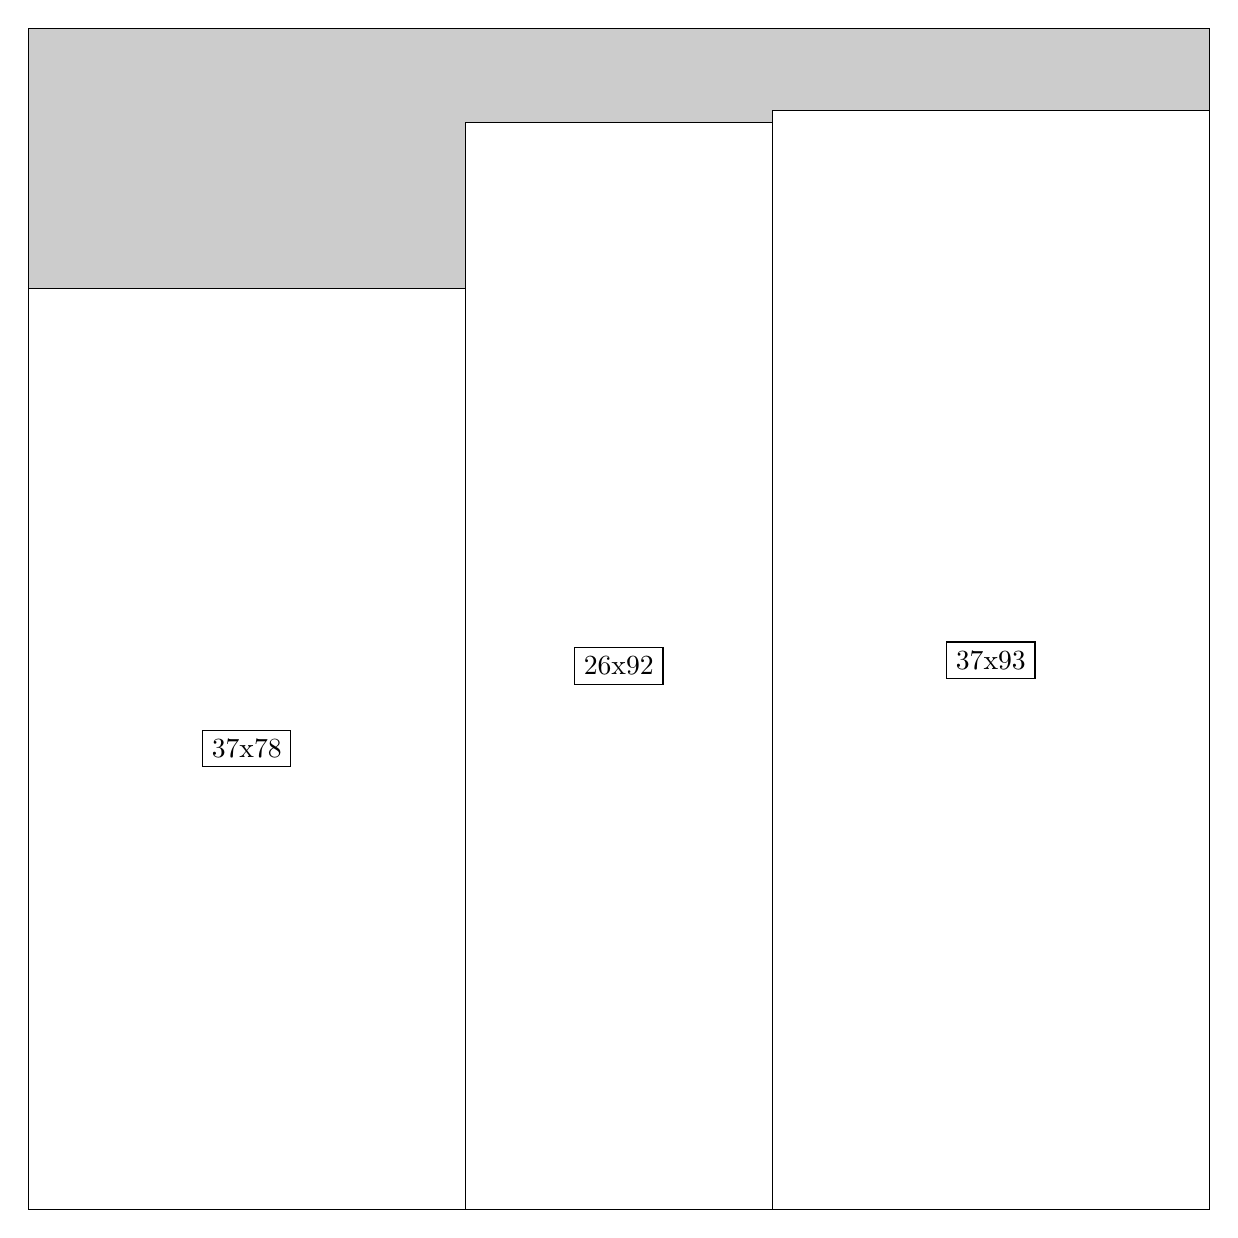
\begin{tikzpicture}[shorten >=1pt,scale=1.0,every node/.style={scale=1.0},->]
\tikzstyle{vertex}=[circle,fill=black!25,minimum size=14pt,inner sep=0pt]
\filldraw[fill=gray!40!white, draw=black] (0,0) rectangle (15.0,15.0);
\foreach \name/\x/\y/\w/\h in {37x93/9.45/0.0/5.55/13.95,26x92/5.55/0.0/3.9/13.799999999999999,37x78/0.0/0.0/5.55/11.7}
\filldraw[fill=white!40!white, draw=black] (\x,\y) rectangle node[draw] (\name) {\name} ++(\w,\h);
\end{tikzpicture}


w =37 , h =93 , x =63 , y =0 , v =3441
\par
w =26 , h =92 , x =37 , y =0 , v =2392
\par
w =37 , h =78 , x =0 , y =0 , v =2886
\par
\newpage


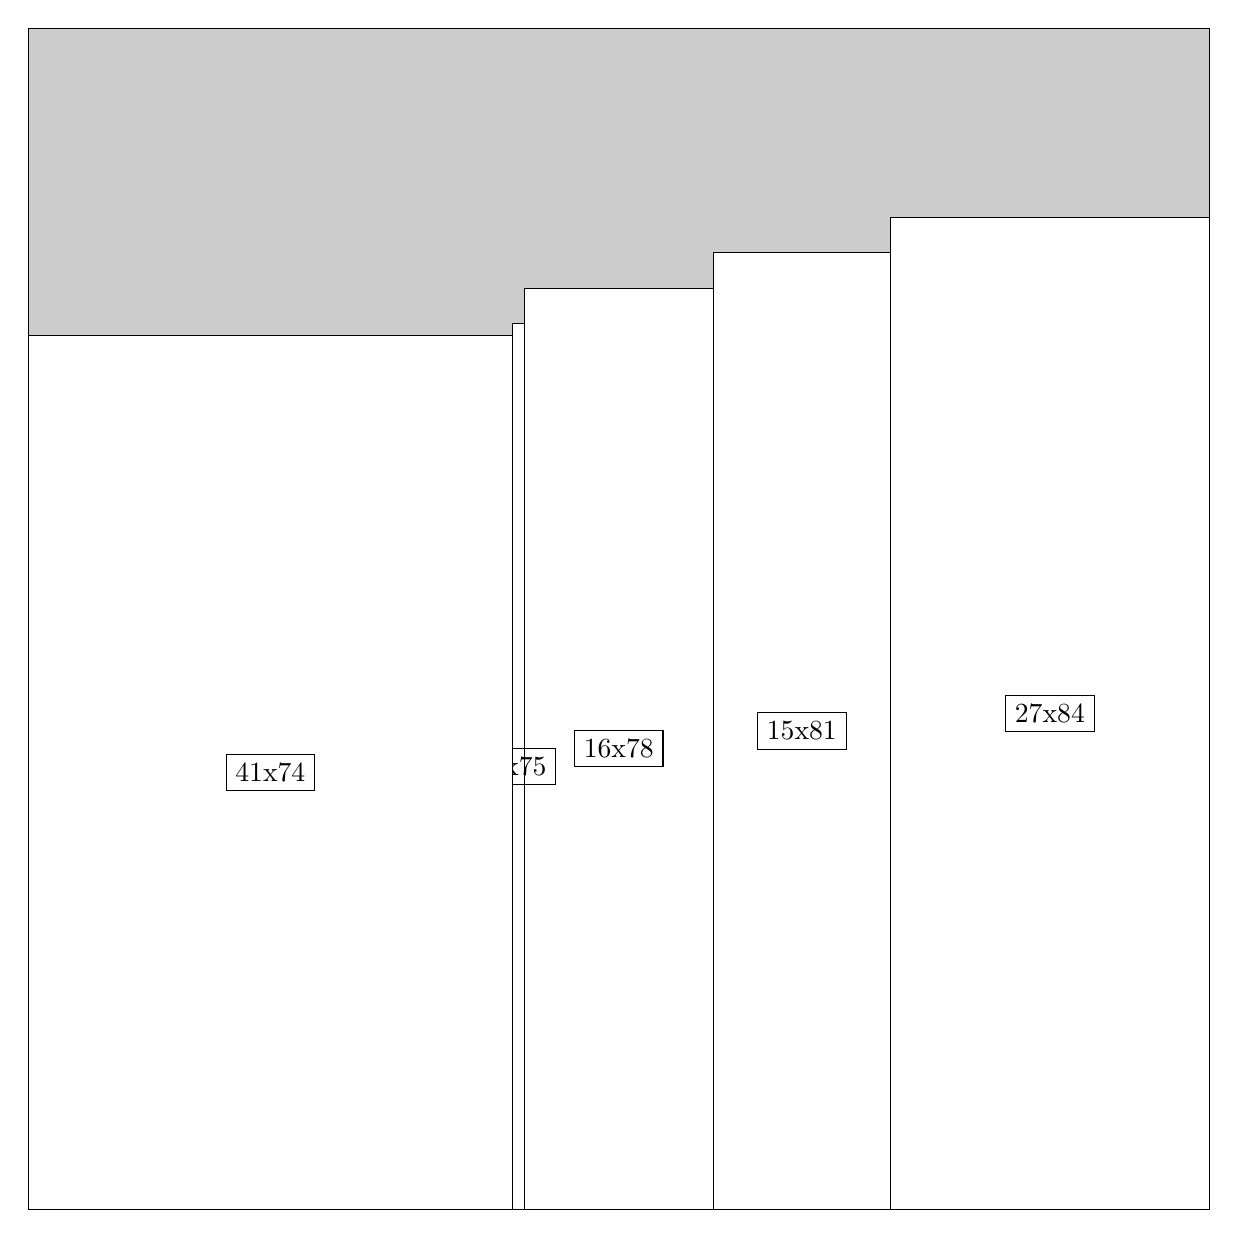
\begin{tikzpicture}[shorten >=1pt,scale=1.0,every node/.style={scale=1.0},->]
\tikzstyle{vertex}=[circle,fill=black!25,minimum size=14pt,inner sep=0pt]
\filldraw[fill=gray!40!white, draw=black] (0,0) rectangle (15.0,15.0);
\foreach \name/\x/\y/\w/\h in {27x84/10.95/0.0/4.05/12.6,15x81/8.7/0.0/2.25/12.15,16x78/6.3/0.0/2.4/11.7,1x75/6.1499999999999995/0.0/0.15/11.25,41x74/0.0/0.0/6.1499999999999995/11.1}
\filldraw[fill=white!40!white, draw=black] (\x,\y) rectangle node[draw] (\name) {\name} ++(\w,\h);
\end{tikzpicture}


w =27 , h =84 , x =73 , y =0 , v =2268
\par
w =15 , h =81 , x =58 , y =0 , v =1215
\par
w =16 , h =78 , x =42 , y =0 , v =1248
\par
w =1 , h =75 , x =41 , y =0 , v =75
\par
w =41 , h =74 , x =0 , y =0 , v =3034
\par
\newpage


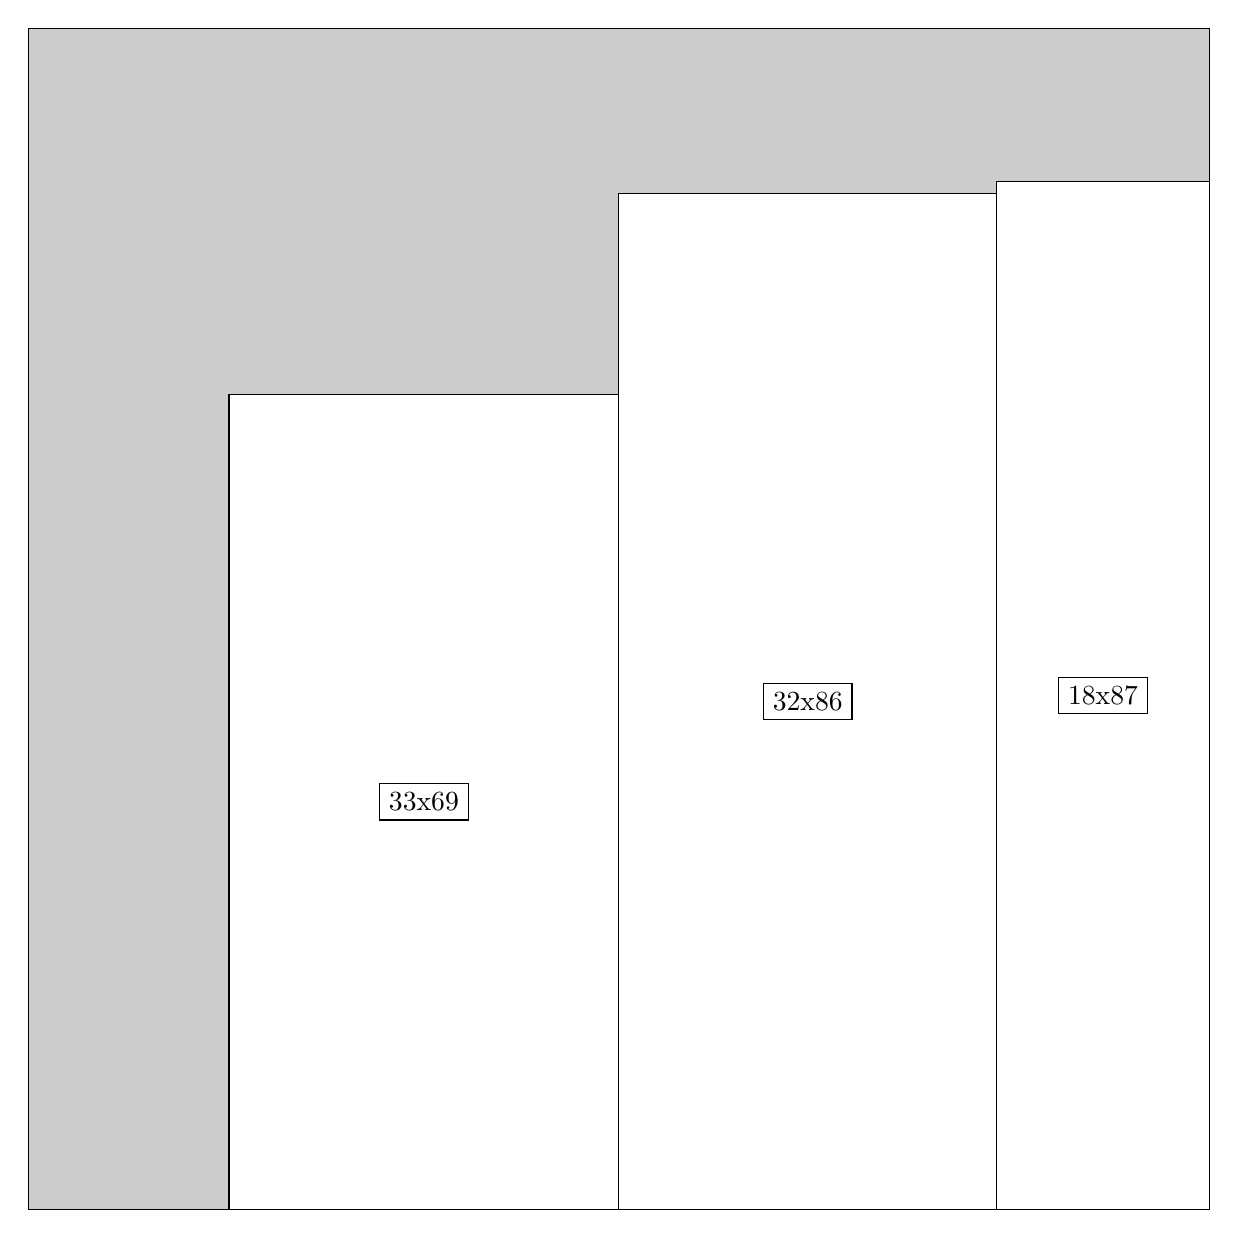
\begin{tikzpicture}[shorten >=1pt,scale=1.0,every node/.style={scale=1.0},->]
\tikzstyle{vertex}=[circle,fill=black!25,minimum size=14pt,inner sep=0pt]
\filldraw[fill=gray!40!white, draw=black] (0,0) rectangle (15.0,15.0);
\foreach \name/\x/\y/\w/\h in {18x87/12.299999999999999/0.0/2.6999999999999997/13.049999999999999,32x86/7.5/0.0/4.8/12.9,33x69/2.55/0.0/4.95/10.35}
\filldraw[fill=white!40!white, draw=black] (\x,\y) rectangle node[draw] (\name) {\name} ++(\w,\h);
\end{tikzpicture}


w =18 , h =87 , x =82 , y =0 , v =1566
\par
w =32 , h =86 , x =50 , y =0 , v =2752
\par
w =33 , h =69 , x =17 , y =0 , v =2277
\par
\newpage


\end{document}